\RequirePackage[2020-02-02]{latexrelease}
\documentclass{ntuthesis}


\usepackage{amsmath, amssymb, amsthm}
\usepackage{bm, bbm}
\usepackage{physics}
\usepackage{natbib}
% \usepackage{newtxmath}
\usepackage{appendix}
\usepackage{caption}    % for subfigure
\usepackage{subcaption} % for subfigure
\usepackage[compact]{titlesec}    % remove redundant spacing
\usepackage{times}
\usepackage{threeparttablex,longtable}
\usepackage{booktabs}
\usepackage{afterpage}  % load the afterpage package
\usepackage[inline]{enumitem}   % can get rid of new line
\usepackage{verbatim}
\usepackage{color}
\usepackage{url}
\usepackage{graphicx}
\usepackage{setspace}
\usepackage{array}
\usepackage{wallpaper}
\usepackage[hidelinks]{hyperref}
\usepackage[printwatermark]{xwatermark}
\usepackage[capposition=top]{floatrow}
\usepackage{chngcntr}
\newcommand{\BL}{\emph{Bitcoin Law}}
\newcommand{\chivo}{\emph{Chivo Wallet}}
\newcommand{\BC}{\emph{Bitcoin City}}

\DeclareMathOperator*{\argmin}{arg\,min}

\newcommand{\refeq}[1]{Equation~({\ref{#1}})}
\newcolumntype{H}{>{\setbox0=\hbox\bgroup}c<{\egroup}@{}}


\counterwithout{equation}{chapter}
\counterwithout{figure}{chapter}
\counterwithout{table}{chapter}
% Using the tex-text mapping for ligatures etc.
\defaultfontfeatures{Mapping=tex-text}
% Set the default fonts
\setmainfont{Times New Roman}
\setCJKmainfont[AutoFakeBold=true,AutoFakeSlant=true]{標楷體}
%\setCJKmainfont[BoldFont={粗楷體},ItalicFont={斜楷體}]{標楷體}

\theoremstyle{definition}
\newtheorem{definition}{Definition}

\ifdefined\firstpage

  \def\withwatermark{1}
  \ifdefined\withwatermark
    \newsavebox\mybox
    \savebox\mybox{\tikz[opacity=0.5]\node{
\includegraphics{watermark.pdf}};}
    \newwatermark*[allpages,xpos=6.1725cm,ypos=10.5225cm,scale=0.5]{\usebox\mybox}
  \fi

  % digital object identifier
  \ifdefined\withdoi
    \insertdoi
  \fi
\fi

\makeatletter
\AtBeginDocument{
  \hypersetup{
    pdftitle={\@titleen},
    pdfauthor={\@authoren},
    pdfsubject={\@typeen{} \@classen},
    pdfkeywords={\@keywordsen}
  }
}
\makeatother

% Your information goes here
% author: Tz-Huan Huang [http://www.csie.ntu.edu.tw/~tzhuan]

% ----------------------------------------------------------------------------
% "THE CHOCOLATE-WARE LICENSE":
% Tz-Huan Huang wrote this file. As long as you retain this notice you
% can do whatever you want with this stuff. If we meet some day, and you think
% this stuff is worth it, you can buy me a chocolate in return Tz-Huan Huang
% ----------------------------------------------------------------------------

% Syntax: \var{English}{Chinese}
\university{National Taiwan University}{國立臺灣大學}
\college{College of Social Science}{社會科學院}
\institute{Department of Economics}{經濟學系}
\title{Examining the Chinese Debt-Trap Diplomacy}{檢視中國債務陷阱}
\author{Chia-Wei Chen}{陳家威}
\studentid{R10323045}
\advisor{Tai-kuang Ho, Ph.D.}{何泰寬 博士}
\defenseyear{2023}{112}
\defensemonth{July}{7}
\defenseday{12}
\doi{doi:10.6342/NTU2017XXXXX}
\keywords{Debt-Trap Diplomacy, Belt and Road Initiative, Sovereign Debt, Optimal Default}{債務陷阱外交、一帶一路、主權債務、最適違約決定}


\titleformat{\chapter}                      % 設置 Chapter 格式
{\Huge\bfseries}                            % 定義 format
{Chapter~\thechapter:~}              		        % 定義 label
{1em}                                       % 定義 sep
{} 
\begin{document}

\frontmatter

\makecover

\ifdefined\excludefirstpage

  \def\withwatermark{1}
  \ifdefined\withwatermark
    \newsavebox\mybox
    \savebox\mybox{\tikz[opacity=0.5]\node{
\includegraphics{watermark.pdf}};}
    \newwatermark*[allpages,xpos=6.1725cm,ypos=10.5225cm,scale=0.5]{\usebox\mybox}
  \fi

  % digital object identifier
  \ifdefined\withdoi
    \insertdoi
  \fi
\fi

% \makecertification

% \begin{acknowledgementszh}
感謝\ldots
\end{acknowledgementszh}

\begin{acknowledgementsen}
I'm glad to thank\ldots 
\end{acknowledgementsen}

% \begin{abstractzh}
關於中國在「一帶一路」倡議下向接受國家提供的過度貸款是否導致這些國家陷入高度債務並最終陷入「債務陷阱」的爭議仍然存在。本論文旨在通過運用一個主權債務模型的校準,從實證角度對這個議題進行考察。具體而言,本研究聚焦於兩個在中國戰略上具有重要地位的國家 --- 斯里蘭卡和巴基斯坦。

研究結果確認了這兩個國家在接受大量貸款後確實陷入了債務違約的狀態。基於這些結果,本研究提出了兩個債務陷阱的類別,並將斯里蘭卡和巴基斯坦分別歸入不同的類別。這種分類方法為債務陷阱外交的相關文獻提供了客觀的評估和呈現方式。
\bigbreak
\noindent \textbf{關鍵字:}{\, \makeatletter \@keywordszh \makeatother}
\end{abstractzh}

\begin{abstracten}

    Ongoing debates remain surrounding whether the excessive loans provided by China under the Belt and Road Initiative lead to high indebtedness and eventual ``debt traps'' for recipient countries. This thesis empirically examines this topic through the calibration of a sovereign debt model. Specifically, the study focuses on two strategically important countries --- Sri Lanka and Pakistan.
    The research findings validate the notion that these two countries indeed fell into the default set once they received substantial loan amounts, allowing for two categories of debt traps into which Sri Lanka and Pakistan reside. This categorization offers an objective assessment and presentation method within the literature on debt-trap diplomacy.
    \bigbreak
\noindent \textbf{Keywords:}{\, \makeatletter \@keywordsen \makeatother}
\end{abstracten}

\begin{comment}
\category{I2.10}{Computing Methodologies}{Artificial Intelligence --
Vision and Scene Understanding} \category{H5.3}{Information
Systems}{Information Interfaces and Presentation (HCI) -- Web-based
Interaction.}

\terms{Design, Human factors, Performance.}

\keywords{Region of interest, Visual attention model, Web-based
games, Benchmarks.}
\end{comment}


% \tableofcontents
% \listoffigures
% \listoftables

\mainmatter


\chapter{Introduction}
As China's economic influence continues to grow, its lending practices to developing countries have come under scrutiny.
The concept of ``debt-trap diplomacy'' (hereinafter DTD), whereby China extends excessive loans to countries in exchange for political or economic concessions, has become a topic of heated debate \citep{Chellaney_2017}.
While some argue that the debt-trap problem poses a significant threat to the economic and political stability of vulnerable countries, others contend that it is overstated.

From the political science aspect, an analysis from the Belfer Center for Science and International Affairs states that China utilizes DTD as a technique to achieve strategic objectives, such as projecting power across South Asian trading routes, undermining regional opposition to its South China Sea claims, and supporting its naval efforts to break out into the Pacific \citep*{Parker2018}.
Critics of this phenomenon argue that claims of DTD are often exaggerated or based on incomplete information. For example, \citet*{Brautigam-meme-2020} argues that the debt-trap is based on a flawed understanding of Chinese lending practices and the histories of the target countries, and that China is not strategically pursuing the DTD on developing countries.

The opacity in Chinese lending practices has been a longstanding challenge in the analysis of the DTD problem \citep*{Horn-Reinhart-Trebesch-21}.
The lack of transparency in the Chinese lending system, whereby loan terms, conditions and collateral requirements are not always disclosed to the borrowers, makes it difficult for economists and policymakers to fully grasp the magnitude of the issue.
Therefore, it has been challenging to assess the sustainability of debts of borrowing countries and their ability to service their obligations, as well as the potential impact of China's lending practices on the economy of low income developing countries (LIDC), especially those in the Belt and Road Initiatives (BLI).
As a result, recent studies on whether DTD is a myth have primarily been conducted normatively in the field of political science, rather than a positive economics analysis~\citep[See, e.g.,][]{Himmer2023-vn,Chen2020-eo}.

However, with the emergence of new and detailed data on Chinese lending practices, recent studies have begun to shed light on the nature and implications of the China debt.
In this thesis, I aim to shed light on whether a country fell into the debt-trap by applying a new and detailed data provided by \citet*{Horn-Reinhart-Trebesch-21}, hereinafter referred to the ``HRT database'', on the sovereign debt model proposed by \citet*{Na-18}, to provide insights into the sustainability of the debt of borrowing countries.
By calibrating the model for a particular country, a set of tradable-output levels which would cause the country to default could be obtained, given its current debt level. Following the approach of \citet{Hinrichsen_2020-chapter4}, this set is presented graphically with each data point on the space representing a debt-output pair for a specific year. This visual representation allows for an examination of whether the country has been in the default zone but has managed to avoid default due to other enforcement mechanisms, in this case might be the political leverage from China.

It requires a lot of work to calibrate all countries to match the model, therefore it is optimal to narrow down the sample countries to those that provides the most insight on the DID issie. I consider countries
\begin{enumerate*}
    \item that is constantly receiving loans from other international institutes,
    \item that indicates an increasing amount of debt from China that eventually exceeds other creditors, and
    \item in which China launches large infrastructure programs.
\end{enumerate*}
% \citet*{Hurley19-8-debt-trap} examines the dept-to-GDP ratio versus the share of China's debt, and identifies eight
% countries\footnote{
%     These countries are Djibouti, Kyrgyzstan, Laos, the Maldives, Mongolia, Montenegro, Pakistan, and Tajikistan}
% that are particularly risky.
In particular, the default sets for Sri Lanka and Pakistan are examined in this thesis. I will further provide the basic backgrounds for the two sample countries in later sections.

\section{HRT Database}
China's official external lending is predominantly undertaken by state-owned entities and the government itself\footnotemark{}. However, unlike other major economies, the Chinese government does not report or publish any data on its official international lending or outstanding overseas debt claims. This lack of transparency creates challenges for rating agencies, as official lending to sovereigns is not a regular part of their activities. Moreover, China is not a member of the Paris Club, which tracks sovereign borrowing from official bilateral creditors, and does not divulge data on its official flows with the OECD's Creditor Reporting System \citep*{Horn-Reinhart-Trebesch-21}.
\footnotetext{These include China's state-owned policy banks, such as China Development Bank (國家開發銀行, CDB) and China Export-Import Bank (中國進出口銀行, Ex-Im), as well as China's state-owned commercial banks such as Industrial and Commercial Bank of China (中國工商銀行, ICBC) or Bank of China (中國銀行, BoC)}

\citet*{Horn-Reinhart-Trebesch-21} combines a variety of sources to construct a consensus database of Chinese official loans.
The HRT database spans from 1949, the establishment of the People's Republic of China, to 2017. It contains a granular dataset of 2151 loans and 2824 grants with information such as the creditor agent, borrower type, commitment, maturity, etc. It also provides an aggregate panel data of the external debt to China for each country.
\begin{figure}[t]
    \centering
    \begin{subfigure}[t]{0.45\textwidth}
        \centering
        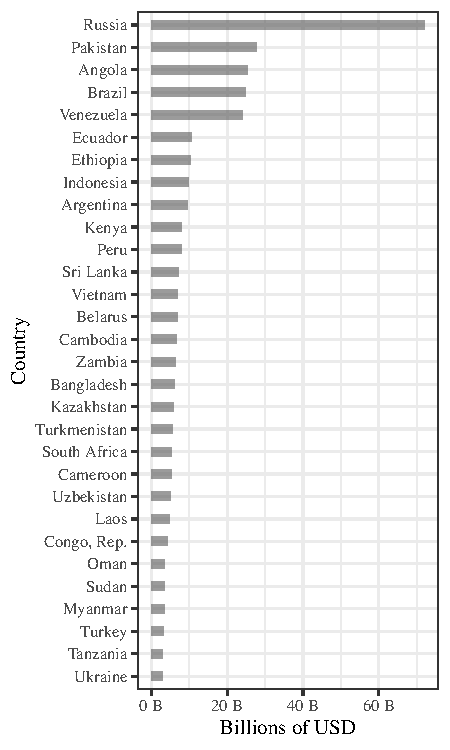
\includegraphics[width = \textwidth]{fig/total_debt.pdf}
        \caption{Top 30 Debtor by Total Debt in USD}
        \label{fig:total-debt-30}
    \end{subfigure}%
    ~
    \begin{subfigure}[t]{0.45\textwidth}
        \centering
        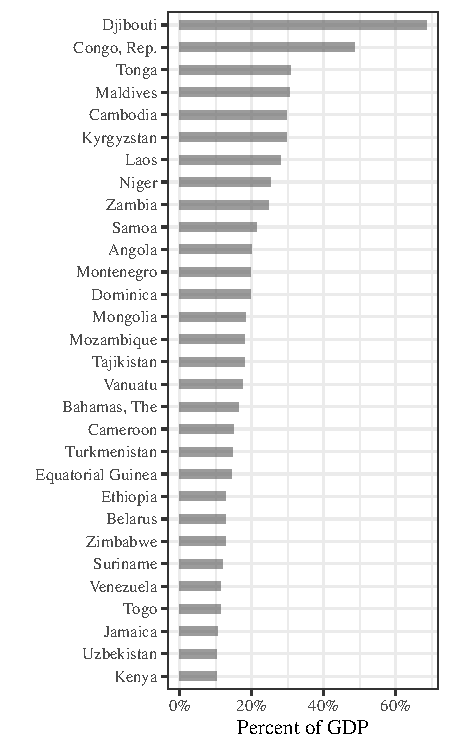
\includegraphics[width = \textwidth]{fig/perc_debt.pdf}
        \caption{Top 30 Debtor by Dept-to-GDP Ratio}
        \label{fig:perc-debt-30}
    \end{subfigure}
    \caption{Debt to China Statistic by Country in 2017}
    \label{fig:Country-Agg}
    \floatfoot{Source: HRT Database \citeyearpar{Horn-Reinhart-Trebesch-21} \\
    Note: The figure on the left presents the top 30 countries in amount of total external debt to China in 2017. The figure on the right compares by the China-debt-to-GDP ratio.}
\end{figure}

The top 30 countries with the largest debts to China's official creditors are displayed in \autoref{fig:total-debt-30}. Notably, Russia owes China over \$70 billion, while Pakistan's debt amounts to \$27 billion, both topping the list. Brazil and Venezuela are among the top 10 countries with the highest debt to China in Latin America. Contrary to what many people believe, African countries have not borrowed much from China. However, if we consider the ratio of Chinese debt to GDP in \autoref{fig:perc-debt-30}, some African countries appear to be highly indebted to China. Djibouti, for instance, has an alarming ratio of 68.5\% of its GDP consisting of Chinese debt, while Tonga, Niger, and Zambia have ratios exceeding 10\%.
\begin{figure}
    \centering
    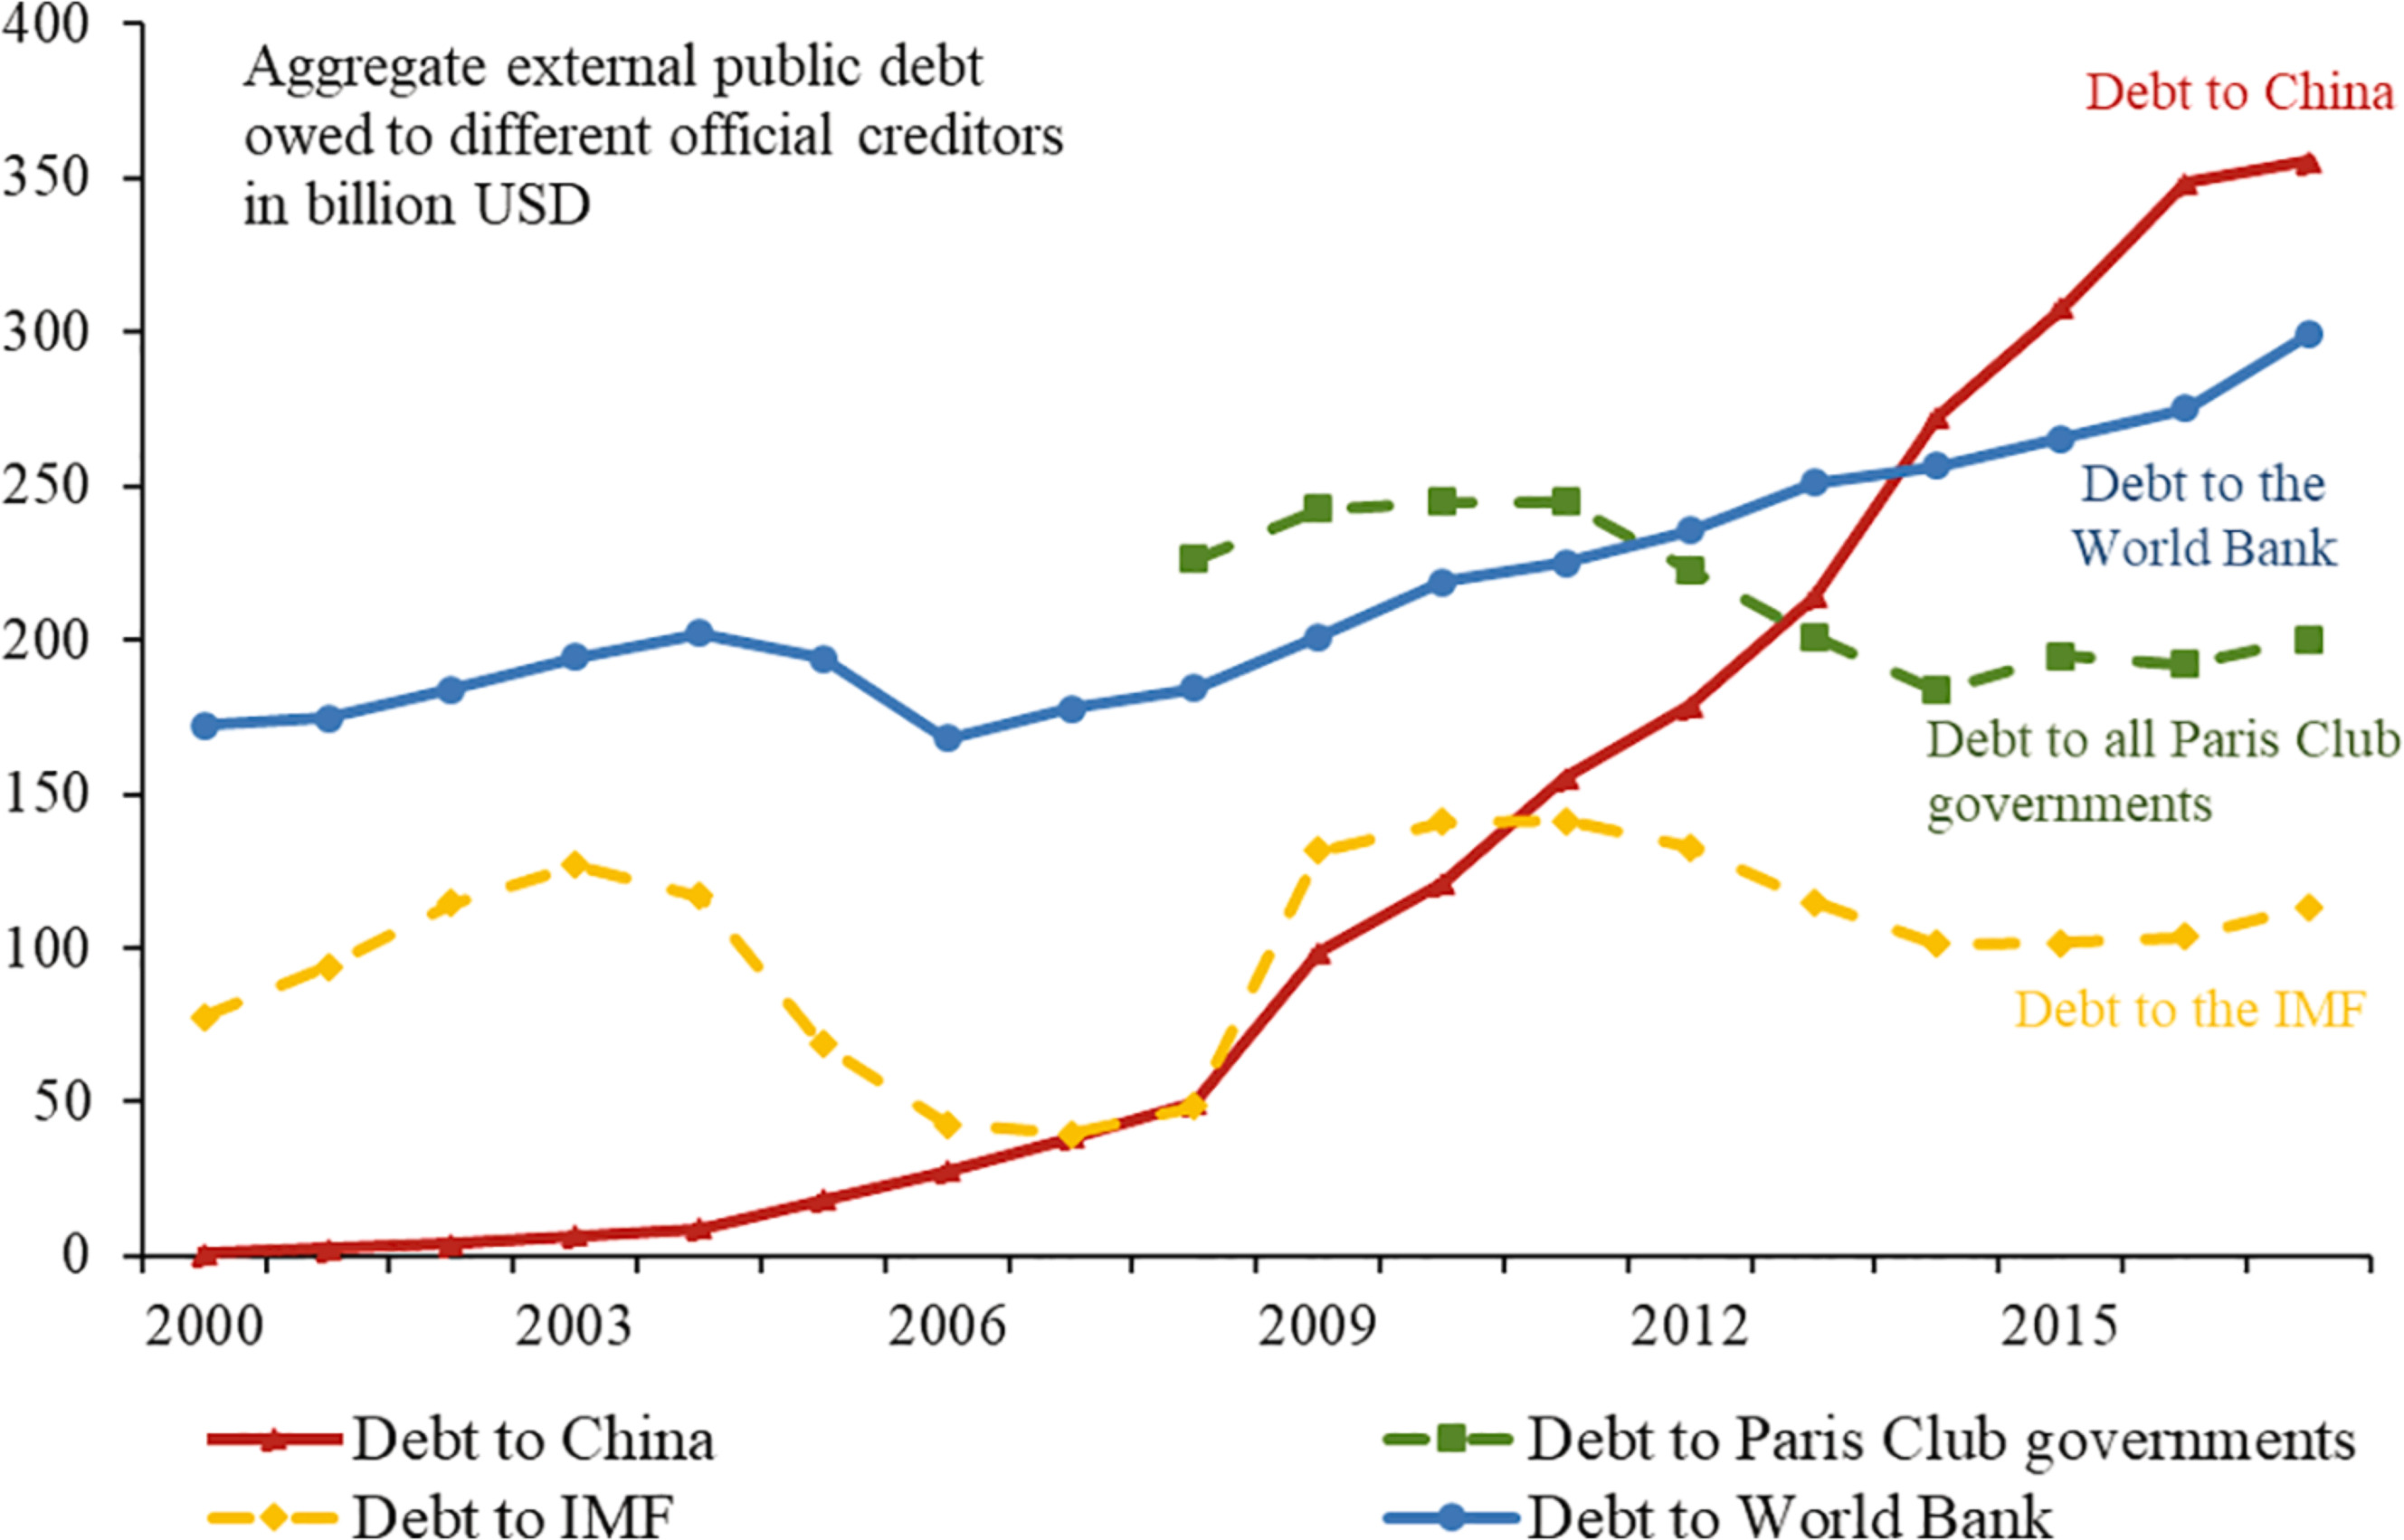
\includegraphics[width = 0.7\textwidth]{fig/temp-external-all-creditor.jpg}
    \caption{Change of Aggregate Public Debt for Different Official Creditors}
    \label{fig:debt-ts}
    \floatfoot{Source: HRT Database \citeyearpar{Horn-Reinhart-Trebesch-21} \\
    Note: The figure shows the change in the aggregate external public debt that the developing countries owed to different official creditors. These include China, World Bank (excluding China), IMF, and all 22 Paris Club governments. It is obvious that China had become the largest official creditors in the world according to the estimation of \citet*{Horn-Reinhart-Trebesch-21}.}
\end{figure}

A main finding in \citet*{Horn-Reinhart-Trebesch-21} is that China had become the world's largest creditor to developing countries after 2013, surpassing the amount of World Bank. \autoref{fig:debt-ts} shows the change of the total amount of debt from different main creditors, including China, World Bank\footnote{Including the International Development Association (IDA) and the International Bank for Reconstruction and Development (IBRD) }, IMF, and the aggregation of all countries in the Paris Club. The debt amount started to rise rapidly after 2000, when the China government launched the ``Go Out Policy'' in 1999. In 2017, the debt to China had reached \$355 billion, while the debt to World Bank was \$300 billion.


This database allows researchers to obtain the true amount of total debt of a country, and gauge the amount of debt that is considered superfluous and onerous for it.
For the next section, I briefly explain the two countries I will examine in my thesis, and demonstrate the importance of choosing it as a benchmark example.

\section*{Sri Lanka}
In the original article where the terminology ``Debt-trap Diplomacy'' was coined, \citet{Chellaney_2017} specifically mentioned the predicament faced by the Sri Lankan government. He argues that the Chinese government supported large infrastructure projects in Sri Lanka and provided heavy loans to their government, and as the project eventually failed to repay the debt, the country is then ensnared in the concessions to China. \autoref{fig: sri-lanka-debt-ts} shows the change in composition of the creditors to Sri Lanka.

The issue of the Hambantota port is regarded as a typical example of a debt-trap for some scholars~\citep*{Moramudali_2020}.
The construction of the port was initiated in 2007 and entrusted to the state-owned Chinese companies --- China Harbour Engineering Company and Sinohydro Corporation. The project was valued at \$361 million, of which Exim Bank financed 85\% at a yearly interest rate of 6.3\%\footnote{From AidData Project ID \#33409, ``China Eximbank provides \$306.7 million buyer's credit loan for Phase I of Hambantota''}.


China's involvement in Sri Lanka's infrastructure development was facilitated by President Mahinda Rajapaksa, during which China became Sri Lanka's leading investor and lender. This gave China significant diplomatic leverage over Sri Lanka. 
However, when Rajapaksa was unexpectedly defeated in the early 2015 election by Maithripala Sirisena, who campaigned on the promise to extricate Sri Lanka from the Chinese debt trap, work on major Chinese projects was suspended.

However, Sri Lanka's government was already on the brink of default, and Sirisena eventually acquiesced to a series of Chinese demands\footnotemark{}, including the sale of an 70\% stake in the Hambantota port to China Merchants Port (CM Port) and a 99-year lease.
\footnotetext{This narrative origins from \citet*{Chellaney_2017}. \citet*{Brautigam-meme-2020}, however, provides a different narrative. She mentioned that ``\emph{The proceeds were used to increase Sri Lanka's
US dollar reserves in 2017-18 with a view to the repayment of maturing international sovereign bonds \dots Therefore, the sale of Hambantota was originally a fire sale designed to raise money to deal
with larger debt problems.}''}
Notably, as argued by \citet*{Moramudali_2019}, the lease did not write off the loans obtained to construct Hambanota port. The proceeds from the lease were used to boost the country's dollar reserves in 2017-18, especially in preparation for the large amount of external debt that needed to be serviced when international sovereign bonds matured in early 2019. This means that the lease is not a debt-equity-swap, as common narratives elaborated \citep*{Moramudali_2020}.
Sri Lanka eventually declared a suspension on payment on most foreign debt from Aril 12, 2022. Whether Sri Lanka was indeed already under the extreme ``brink of default'' during 2015 is a major gap in the literature of sovereign default that has not yet been investigated.

\section*{Pakistan}
Similar to Sri Lanka, we observe the abrupt increase on the debt to China, as it already has a relatively high debt to other official creditors. \autoref{fig: pakistan-debt-ts} shows the change in composition of creditors to Pakistan. 
Pakistan is the centerpiece of the China Pakistan Economic Corridor (CPEC), a 3000 km corridor that connects China with the Arabian sea.
CPEC serves as an important network as it reduces the passage for China's energy import from the Middle Eastern countries \citep*{CPEC-wiki}.

China has launched enormous amounts of infrastructure in Pakistan after 2015. These items include a deep water port, road and rail lines, and most importantly, energy sector projects. Up to 2018, the estimation of the total value of projects under the CPEC is \$62 billion, out of which around \$33 billion is allocated for energy projects~\citep*{Hurley19-8-debt-trap}. China is expected to finance about 80 percent of this amount. The private investments for energy projects in Pakistan will be financed by the Exim Bank of China at an interest rate of 5-6\%. 
Private Independent Power Producers (IPP) will be responsible for constructing the energy projects under CPEC, instead of the governments of China or Pakistan. In turn, the government of Pakistan will be legally bound to buy electricity from these companies at rates that were agreed upon before.
However, despite this significant investment, some projects have already been cancelled, such as three major road projects that were cancelled at the end of 2017 \citep*{Hurley19-8-debt-trap}.

In the case of Pakistan, the sudden increase of debt to China draws the attention of researchers and journalists. For example, a report from the Financial Time titled ``Pakistan is on the brink'' states that Pakistan is following Sri Lanka into default. Given the recent frequent analogy drawn between Pakistan and Sri Lanka, it is essential to analyze Pakistan from the perspective of the sovereign default model.

  \label{ch:intro}
\chapter{Literature Review} \label{ch:lit}
\section{Debt-Trap Diplomacy}
Whether the debt-trap diplomacy is just a conspiracy used as an instrument for western countries to justify their political strategy or is in fact causing stress on the receiving counties intentionally has continuously seen great debates and arguments.

%% +1
The term ``debt-trap diplomacy'' was first coined by \citet{Chellaney_2017}, who states that the infrastructures supported financially by the China government in Sri Lanka are burdensome and causing Sri Lanka, as well as other small and poor countries, to endure the unsustainable loans, forcing them to cede strategic leverage to China.
%% +2, +4, +5
From a political aspect,
researchers from the Belfer Center for Science and International Affairs propose that China may pursue three main strategic objectives using this approach \citep*{Parker2018}.
These objectives include:
\begin{enumerate*}[label = (\roman*)]
    \item expanding its ``String of Pearls'' to address the ``Malacca Dilemma'' and extend its influence along crucial South Asian trade routes,%
    \footnote{
        The Strait of Malacca, located between Malaysia and Indonesia, is one of the busiest and most critical shipping routes in the world, connecting the Indian Ocean and the Pacific Ocean.
        The ``Malacca Dilemma'' refers to the strategic vulnerability faced by China due to its heavy dependence on the Strait of Malacca for maritime trade and energy imports \citep*{Parker2018}.
    }
    \item destabilizing and fragmenting the regional coalition led by the United States that challenges China's claims in the South China Sea, and
    \item facilitating the People's Liberation Army Navy (PLAN) in advancing beyond the "Second Island Chain" and into the open waters of the Pacific Ocean.%
    \footnote{
        The Second Island Chain encompasses a collection of islands, such as the Bonin Islands and Volcano Islands of Japan, the Mariana Islands (notably Guam), the western Caroline Islands, and extending towards Western New Guinea. It serves as the delineation of the eastern maritime boundary of the Philippine Sea, while also incorporating Guam, an American overseas territory housing a strategically fortified military base
        \citep{Vorndick-Island-chian-18}.
    }
\end{enumerate*}
% +3
This is considered as the reshaping of ``soft'' infrastructure that China is hoping to enhance \citep{Jonathan-Hillman-18}.

% +?
A common criticism concerning the loans from China is that the terms and conditions are typically not transparent compared to other creditors in order to encourage those debtor countries' dependency to China \citep{tillerson2018us}. For example,
an analysis on the contract of China's long foreign lending suggests that the terms of these agreements feature unusual confidentiality clauses, seek advantages over other creditors through collateral arrangements, and potentially grant influence over debtors' policies \citep{Gelpern-22}.
The authors reveal that the contracts signed with Chinese state-owned entities after 2014 frequently contain extensive clauses to maintain confidentiality that impose broad obligations on the debtor to keep contract details and related information undisclosed. Furthermore, about 30\% of these agreements require the borrowing country to establish a dedicated bank account, typically controlled by the lender, as a form of collateral for debt repayment. These revenue accounts, uncommon in sovereign lending, restrict the borrowing country's authority over its own finances. Additionally, compared to other types of debt contracts, China's loans agreements more commonly include cross-default clauses, allowing lenders to demand immediate repayment (called an \emph{acceleration}) if the borrower defaults on other lenders.%
\footnote{
    These agreements allow China to jump the ``seniority queue'', and hence making debt to China de facto seniority debts \citep{Chen-Muyang-23-china-debt-seniority}.
}
These contract characteristics, along with their creative design to manage credit risks and enforcement hurdles, portray China as a powerful and commercially astute lender to developing nations.

There are several studies regarding the estimation of debt vulnerability caused by China's loans. \citet*{Hurley19-8-debt-trap} evaluate the debt sustainability in BRI countries by examining their dept-to-GDP ratio versus their share of China's debt. Following the threshold of 50-60\% rising debt-to-GDP ratio constructed by \citet{Chudik-15}, they identify eight
countries that are particularly risky.\footnote{
    These countries are Djibouti, Kyrgyzstan, Laos, the Maldives, Mongolia, Montenegro, Pakistan, and Tajikistan.}
\citet*{Bandiera-Vasileios-BRI-debt} examine the impact of investment and infrastructure projects under BRI on the debt-to-GDP ratios of recipient countries. The authors analyze the growth effects of BRI investment and estimates the potential increase in debt vulnerabilities for certain countries through a model-based growth projection. The findings suggest that approximately 28\% of BRI investment recipient countries, consisting of 7 low-income developing countries and 5 emerging markets, are expected to face increased debt vulnerability in the medium term, while 37\% of countries, including 5 low-income developing countries and 6 emerging markets, may experience a rise in their debt-to-GDP ratio due to BRI investment and financing in the long term, with 8 of them being vulnerable to changes in financing costs.


In stark contrast, critics of the ``debt-trap diplomacy'' narrative often argue that the benefit of China's lending on the receiving country is neglected, and state that the concerns are often exaggerated.
% -3
\citet*{Eom-18} argue that Chinese loans did not play a significant role in causing debt distress in Africa. They identify 17 African low-income  countries that were and under high risk of debt distress and find for less than half (8) of them, their levels of debt to China were relatively small compared to their total external debt, and that the debt distress was caused primarily by other conflicts in the nation; six other countries had higher loans from China, but also to other official creditors; and in only three countries, Chinese loans were the main contributions to the debt distress.
% -4

\citet*{Brautigam-meme-2020} indicates that debtor countries have voluntarily accepted Chinese loans and report positive experiences, suggesting that concerns over Chinese infrastructure funding are exaggerated, as many view China as an appealing economic model and development partner.
In the case of Sri Lanka, \citet*{Brautigam-meme-2020} also argues that the project of Hambantota Port was the concept of former President Mattala Rajapaksa, and that Chinese banks have shown willingness to assist their restructuring of existing loans.
% -5
The Rhodium Group presents 40 cases of China's external debt renegotiations, and finds that not only are asset seizures a rare occurrence, but China is limited in its leverage during negotiation due to external events such as change in leadership \citep*{Rhodium-DTD-19}.

Governments of indebted countries often defend their own loan decisions. The Minister of Finance of the Trinidad and Tobago, for instance, argued that choosing a loan without the need for retrenchment, currency devaluation, or other adverse measures, especially when the interest rates are similar, is an obvious and favorable choice.\footnote{Loop News ``Imbert: Choosing between IMF, Chinese loan a `no-brainer,'''June 15, 2021.}

\section{Sovereign Debt Model}
Sovereign debt models under the Eaton-Gersovitz framework have been widely used to analyze default decisions driven by reputation and sanction \citep*{Eaton-Gersovitz-81}.
Several important features are included in the framework to replicate important stylized facts not captured under the benchmark model of Eaton-Gersovitz.
For instance,
\citet{Aguiar-Gopinath-06} and \citet{Arellano-08} take into consideration the risk premium in the market price of debt. As a result, country spread, defined by the difference between the country's net interest rate and the world risk-free interest rate, can be accounted for quantitatively.
\citet{Na-18} further investigate the role of government's optimal policy under wage rigidity in a decentralized economy to study the \emph{Twin Ds} phenomenon. They find that being able to freely set the optimal taxation rate and devaluation rate improves the welfare of a country by reducing unemployment, which provides further incentive for a country to default.

\citet*{Mendoza-Yue-12} endogenize output cost by combining sovereign default and business cycle, thus offering a microfoundation for the ad-hoc assumption of output costs during default episodes in \citet{Arellano-08}. The firm in the economy faces a working capital constraint that amplifies the effect caused by a shock in total factor productivity.
\citet*{Chatterjee-12} consider the fact that sovereign bonds have long and short maturities, and the authors extend the model such that their maturity is realized with a probability.

Seniority of debt is another popular topic in recent literature. Seniority is the priority of a debt contract among all debts. An empirical study by \citet*{Schlegl-Trebesch-Wright-19} shows that private creditors are often paid first, compared to bilateral official creditors, and multilateral institutions (IMF and World Bank) are indeed senior creditors. \citet*{Chatterjee-15-seniority} propose a model to analytically track the seniority of debts. \citet*{Ho-Ritschl-23} extend the Eaton-Gersovitz model to include both senior and junior debts, representing either commercial debts or war reparations. The assignment of seniority for the different debts can then be switched, which the authors refer to as ``seniority reversal.''

Another important stylized fact regarding sovereign defaults is that these episodes are in general partial defaults, contrary to the assumption that a country resets its debt levels after a temporary exclusion from the international financial market \citep[see][]{Sturzenegger-Zettelmeyer-08,Cruces-Trebesch-13}. The fraction that a country chooses to default is called \emph{haircuts} and is usually determined through debt renegotiations.
\citet{Yue-10} combines the benchmark Eaton-Gersovitz model with a Nash bargaining game model to simultaneously explain default and debt negotiations. The author proves that the bargaining power has a great impact on debt recovery rate and bond spread.
\citet{Bi-08} incorporates the Eaton-Gersovitz model with a stochastic bargaining model to explain why delays in debt negotiation can actually be beneficial.
However, empirical data show that debt does not necessarily drop following a restructuring; debt during the episode in fact increases first, creating a hump-shaped dynamic. \citet{Arellano-23-partial-default} emphasize this stylized fact and propose a model and accounting framework that explains the phenomenon. \citet{sovereign-debt-review-yue-19} provide a comprehensive review of the literature on sovereign debt.


A rich body of literature examines default episodes using calibration on Argentina \citep{Arellano-08, Schmitt-Uribe-16,Mendoza-Yue-12,Na-18}. \citet*{Hinrichsen_2020-chapter4} examines the effect of war reparations on countries' default set using data from France in the 1870s, Germany in the 1930s, and Finland in the 1940s. \citet*{Ho-Ritschl-23} investigate transfer protection in the Dawes Plan by calibrating the German economy during the 1920s.
\chapter{Analytic Model} \label{ch:model}
International debt often lacks perfect enforcement, and governments hold the decision of whether to repay the debts or default, based on the comparison of future values \citep*{Eaton-Gersovitz-81}. Therefore, default can be considered an optimal policy for a country that faces unsustainable debt levels. By defaulting, the country avoids the burden of paying interest on the debt, but it also faces the consequence of being excluded from the international credit market for a period of time. As a result, the country would have to rely solely on its own financial resources until it regains access to international credit markets.
Moreover, studies have pointed out that sovereign debt defaults are often accompanied by a devaluation of the currency; \citet*{Reinhart02} refers to this phenomenon as ``Twin Ds.''
Empirical analysis by \citet*{Na-18} further observes that the devaluation rate often decreases after the time of default, suggesting that the Twin Ds phenomenon is the joint result of an optimal policy.
They proposed a model that incorporates two key frictions: limited commitment to repay external debts and downward nominal wage rigidity.
It is a decentralized version of the Eaton-Gersovitz sovereign debt model.
The model predicts that default will occur only after a series of increasingly negative output shocks. Prior to default, domestic absorption experiences a severe contraction, which leads to a decline in demand for labor. However, due to downward nominal wage rigidity, real wages fail to adjust downward, resulting in involuntary unemployment. To prevent this situation, the optimal policy is to devalue the domestic currency, thereby reducing the real value of wages. As a result, both the model and the data show that default episodes are usually accompanied by significant currency devaluations \citep*{Na-18}.

For the sovereign debt model, I closely follow \citet*{Na-18} to replicate the stylized facts about sovereign debt defaults and examine the set of conditions under which default is the optimal decision.
The calibrated model will then serve as a benchmark metric that allows us to investigate whether China has potentially trapped heavily indebted poor counties into default, using the approach proposed by \citet*{Hinrichsen_2020-chapter4}.

\section{Households}
The model assumes that the economy is populated by a large number of representative households who maximize their expected lifetime utility
\begin{equation}
    \label{eq:utility}
    E_0 \sum_{t=0}^\infty \beta^t U(c_t),
\end{equation}
where $\beta \in(0,1)$ denotes the discount factor,
and $c_t$ represents the consumption good, which is composed of
tradable consumption $c_t^T$ and nontradable consumption $c_t^N$.
Assume that $c_t$ follows an aggregate technology
\begin{equation}
    \label{eq:A}
    c_t = A(c^T_t, c^N_t),
\end{equation}
where $A$ is an increasing, concave, and linearly homogeneous function that captures characteristics such as the ratio or elasticity of substitution between tradable and nontradable consumption.
The period utility function $U(c_t)$ follows the standard assumption, which is a strictly increasing and strictly concave function.

Assume that households only have access to the one-period and state non-contingent bond.
The households spend on consumption of tradable and untradable goods, along with their debt which is realized at this period. Their resources consist of labor incomes, dividend incomes, lump-sum transfers, as well as debt incomes. The households are also endowed with tradable goods, which follow a stochastic process.
The budget constraint of the representative household is then
\begin{equation}
    \label{eq:bc}
    P^T_t c^T_t + P^N_t c^N_t + P^T_t d_t =
    P^T_t \tilde{y}^T_t + W_t h_t + (1- \tau^d_t)P^T_t q^d_t d_{t+1} + F_t + \Phi_t,
\end{equation}
where $P^T_t (P^N_t)$ denotes the nominal price of tradable (nontradable) goods, $d_t$ the bond denominated in tradable goods which is due in period $t$, $q_t$ the price of debt to be repaid at $t+1$, $\tilde{y}^T_t$ the endowment of traded goods to the household, $W_t$ the nominal wage, $h_t$ the hours worked, $\tau^d_t$ the tax on debt, $F_t$ a lump-sum transfer from the government, and finally $\Phi_t$ the nominal profits from owning firms.
Households' working hour is bounded by an upper limit
\begin{equation}
    \label{eq:h-constraint}
    h_t \le \bar{h},
\end{equation}
and they take the working hours $h_t$ as given.

The households' problem is to choose $\{c_t, c_t^T, c_t^N, d_{t+1}\}$ such that their utility \eqref{eq:utility} is maximized subjected to the budget constraints \eqref{eq:A} -- \eqref{eq:h-constraint} and the no-Ponzi-game debt limit.
Further denote the relative price of nontradable in terms of tradable goods as $p_t \equiv \frac{P^N_t}{P^T_t}$, we have the following first order conditions
\begin{subequations}
    \begin{align}
        p_t &= \frac{A_2(c_t^T, c_t^N)}{A_1(c_t^t, c_t^N)}\\
        \lambda_t &= U'(c_t)A_1(c_t^T, c_t^N)\\
        (1-\tau_t^d)q_t^d \lambda_t &= \beta E_t \lambda_{t+1},
    \end{align}
\end{subequations}
where $\lambda_t$ is the Lagrange multiplier.

\section{Firms}
Perfectly competitive firms produce nontradable goods $y^N_t$ according to the production technology
\begin{equation}
    \label{eq:production}
    y^N_t = F(h_t),
\end{equation}
where $F$ is strictly increasing and strictly concave. Each firm maximizes its profit by choosing the amount of labor. Profit is given by
\begin{equation}
    \label{eq:profit}
    \Phi_t(h_t) = P^N_t F(h_t) - W_t h_t,
\end{equation}
and the optimal labor demand is then
\begin{equation*}
    P^N_t F'(h_t) = W_t.
\end{equation*}
Dividing both side by the price of tradable goods, and define $w_t \equiv \frac{W_t}{P^T_t}$ as the real wage in terms of tradable goods, the first order condition can be written as
\begin{equation}
    \label{eq:firm-FOC}
    p_t F'(h_t) = w_t.
\end{equation}

\section{Downward Nominal Wage Rigidity}
The key assumption in \citet*{Schmitt-Uribe-16} and \citet*{Na-18} is the downward nominal wage rigidity.
As the wage is unable to be adjusted to a lower level, involuntary unemployment is inevitable, hence the government has the incentive to allow devaluation. The model imposes a lower bound to the growth rate of nominal wage
\begin{equation}
    W_t \ge \gamma W_{t-1}, \qquad \gamma > 0.
\end{equation}
This implies that the growth rate $\frac{W_{t} - W_{t-1}}{W_{t-1}} \ge \gamma - 1$. When this inequality is unbinding ($W_t > \gamma W_{t-1}$), the economy is fully employed ($h_t = \bar{h}$). However, if the condition binds, the economy might have unemployment ($h_t < \bar{h}$). This relationship can be written as the following equation
\begin{equation}
    \label{eq:wage-rigid}
    (\bar{h} - h_t)(W_t - \gamma W_{t-1}) = 0.
\end{equation}


\section{Government}
I assume here, under the lack of enforcement in the international credit market that the government has the option to benevolently free up its domestic balance sheet by choosing to default or not.
Denote $I_t$ as the indicator of whether the government chooses to honor its debt in period $t$. If the government repays in this period ($I_{t} = 1$), then the country will be able to borrow in the following period, and hence $d_{t+1} > 0$. However, if the government chooses to default ($I_t = 0$), then the country will enter the status of financial autarky and is unable to have any sovereign debt in the next period, hence $d_{t+1} = 0$. The above scenario can be written as a slackness condition:
\begin{equation}
    \label{eq:gov-next-debt}
    (1 - I_t)d_{t+1} = 0 .
\end{equation}

To model the duration of financial exclusion, assume that once the country is in bad standing in the international credit market, it can regain a fiscally sound reputation and access to financial markets with probability $\theta \in [0,1)$, and remain in bad standing with probability $1-\theta$. This implies that the country has an average exclusion duration of $\frac{1}{\theta}$ periods.\footnote{
    The expected exclusion period $= \sum_{t=1}^{\infty} t \theta (1-\theta)^{t-1} = \theta  \sum_{t=1}^{\infty} t (1-\theta)^{t-1} = \frac{1}{\theta}$.
}

Assume that the government distributes the proceeds from the debt tax to households as a lump-sum payment. If the government honors the debt, then it repays $d_t$, but if the government decides to default, then it will not make any payments to foreign lenders, and instead will return any payments made by households directly to them. The budget constraint for the government can then be expressed as:
\begin{equation}
    \label{eq:gov-budget}
    f_t = \tau_t^d q_t^d d_{t+1} + (1-I_t)d_t,
\end{equation}
where $f_t \equiv \frac{F_t}{P^T_t}$ is the lump-sum transfer in terms of tradable goods. The right-hand side of the equation states that the transfer to households will include $d_t$ when $I_t = 0$, which is when the country decides to default. Nevertheless, the transfer of debt tax will be zero after default since $d_{t+1} = 0$ when $I_t = 1$, according to Equation \eqref{eq:gov-next-debt}.

\section{Foreign Lenders}
The behavior of foreign lenders is not explicitly modeled in this framework, but as all rational agents, the expected marginal utility of lending to the domestic country must be equivalent to the opportunity cost of funds.
Let $r^*$ represent the opportunity cost for the foreign lenders; this could be the world interest rate. Since $q_t$ is the price of debt that repays one unit of $d_{t+1}$ tomorrow, the return on the debt is $\frac{1}{q_t}$. The lenders take the risk of default into consideration, and hence the expected return will actually be lower. Assume that foreign lenders are risk neutral, this gives
\begin{equation}
    \label{eq:lender}
    \frac{\Pr(I_{t+1}=1 \mid I_{t}=1)}{q_t} = 1 + r^* .
\end{equation}

\section{Competitive Equilibrium}
Under equilibrium, households' consumption equals the production of firms:
\begin{equation}
    \label{eq:nontrade-clear}
    c^N_{t} = y^N_t.
\end{equation}
The tradable goods are purely endowed exogenously under an AR(1) process:
\begin{equation}
    \label{eq:ar1-output}
    \ln(y_t^T) = \rho \ln(y^T_{t-1}) + \mu_t,
\end{equation}
where $\mu_t \overset{\mathrm{iid}}{\sim} \mathcal{N}(0,\sigma_\mu^2)$ is an i.i.d. shock, and $ |\rho| \in [0,1)$ is the autocorrelation parameter.
When the country decides to default, it is in bad standing, and hence it faces an output loss defined by $L(y^T_t)$. The loss function is non-negative and increasing in the tradable goods. The endowment of tradable goods to the household is then:
\begin{equation}
    \label{eq:ytt}
    \tilde{y}^T_t =
        \begin{cases}
        y^T_t  - L(y^T_t) & \text{if } I_t = 0 \\
        y^T_t & \text{otherwise.}
        \end{cases}
\end{equation}
When the country defaults ($I_t = 0$), the endowment decreases.

The price of debt offered by foreign lenders $q_t$ should equal the price of the domestic debt $q^d_t$, but only during good standing:
\begin{equation}
    \label{eq:qq}
    I_t(q^d_t - q_t) = 0.
\end{equation}

The market-clearing condition can be established by combining various equations, including household budget constraints \eqref{eq:bc} and \eqref{eq:h-constraint}, the firm's production function \eqref{eq:production} and profit equation \eqref{eq:profit}, the government's constraint on debt \eqref{eq:gov-next-debt} and lump-sum return \eqref{eq:gov-budget}, and the conditions from \eqref{eq:nontrade-clear}, \eqref{eq:ytt}, and \eqref{eq:qq}.
Eventually, the clearing condition for tradable goods is:
\begin{equation}
    \label{eq:market-clearing}
    c^T_t = y^T_t - (1 - I_t)L(y^T_t) + I_t(q_t d_{t+1} - d_t)
\end{equation}

Assume that the law of one price applies to tradable goods. The foreign currency price of tradable goods is denoted as $P^{T*}_t$, while the nominal exchange rate is represented by $\mathcal{E}_t$. The law of one price states that the price of tradable goods in the domestic currency is equal to the foreign currency price multiplied by the nominal exchange rate.
\begin{equation*}
    P^T_t = P^{T*}_t \mathcal{E}_t
\end{equation*}
This implies that the price of a tradable good should be the same in both domestic and foreign currency terms in an efficient market.

Without loss of generosity, the foreign-currency price of the tradable goods is normalized to 1 ($P^{T*}_t = 1$)
Hence, the nominal price for tradable goods can be expressed as the nominal exchange rate:
\begin{equation}
    \label{eq:price-exrate}
    P^T_t = \mathcal{E}_t.
\end{equation}
For convenience, I also define the devaluation rate of domestic currency as:
\begin{equation}
    \label{eq:devaluation-rate}
    \epsilon_t \equiv \frac{\mathcal{E}_t}{\mathcal{E}_{t-1}} = \frac{P^T_t}{P^T_{t-1}}.
\end{equation}
The conditions are now sufficient to define a competitive equilibrium.
\begin{definition}[Competitive Equilibrium in \citet{Na-18}]
    A competitive equilibrium is a set of stochastic processes $\left\{ c^T_t, h_t, w_t, d_{t+1}, \lambda_t, q_t, q^d_t \right\}$ satisfying:
    \begin{align}
    c^T_t &= y^T_t - (1 - I_t)L(y^T_t) + I_t(q_t d_{t+1} - d_t), \\
    (1 - I_t)d_{t+1} &= 0, \\
    \lambda_t &= U'(A(c^T_t, F(h_t)))A_1(c_t^T, c_t^N),\\
    (1-\tau_t^d)q_t^d \lambda_t &= \beta E_t \lambda_{t+1}, \\
    I_t(q^d_t - q_t) &= 0, \\
    \frac{A_2(c_t^T, F(h_t))}{A_1(c_t^t, F(h_t))} &= \frac{w_t}{F'(h_t)} , \\
   w_t &\ge \gamma\frac{w_{t-1}}{\epsilon_t},\\
   h_t &\le \bar{h},\\
   \left( h_t - \bar{h} \right) \left( w_t - \gamma\frac{w_{t-1}}{\epsilon_t}\right) &= 0, \\
    I_t \left[ q_t - \frac{E_t I_{t+1}}{1+r^*} \right] &= 0,
\end{align}
    given processes $\left\{ y^T_t, \epsilon_t, \tau^d_t, I_t \right\}$ and initial conditions $w_{-1}$ and $d_0$.
\end{definition}
As proven by \citet{Na-18}, if the government is able to set the devaluation rate and the tax on debt freely, then the stochastic process of the variables $\left\{ c^T_t, h_t, d_{t+1}, q_t \right\}$ can be determined by the process of $\left\{ y^T_t, I_t\right\}$ and the initial debt level $d_0$.

As discussed previously, the decision of $I_t$ is an optimal policy for the government due to a lack of commitment to repay debt in the international credit market. Furthermore, the default decision of the government in the next period $t+1$ is also affected by the current decision. To see this argument, first notice that the default decision in $t+1$ is determined by the state variables $\left\{ y^T_{t+1}, d_{t+1} \right\}$. However, $d_{t+1}$ is determined in period $t$, which means that the government in period $t$ understands that it is able to affect the default decision in $t+1$ via the choice of $d_{t+1}$. As $y^T_{t+1}$ follows a first-order Markov process, the expected value of $y^T_{t+1}$ is a function of $y^T_t$, and hence the expected value for the default decision on period $t$ is actually a function of $y^T$ and $d_{t+1}$.

Recall that the price for debt $q_t$ relates to the probability of default in the next period. According to Equation \eqref{eq:lender}, it can be expressed in the contemporary variables:
\begin{equation}
    q_t = q(y^T_t, d_{t+1}).
\end{equation}
On the one hand, this provides economic intuition that the government internalizes the fact that its choice of debt in the next period can affect the price of the debt. On the other hand, this clarifies the dependencies of variables in the value function.


\section{Default Decision}
Following the standard Eaton-Gersovitz framework, this model considers the following three value functions:
value of continuing to repay the debt $v^c$, value of being in good standing $v^g$, and value of being in bad standing $v^b$.

Under the period of being in good financial standing, the value for the government to continue repaying the debt is the maximum value of the utility gained by the households this period, plus the discounted value of being in a good financial standing, subject to the households' budget constraints. Formally,
\begin{equation}
    \begin{aligned}
        v^c(y^T_t, d_t) = \max_{\left\{ c^T_t, h_t, d_{t+1} \right\}} \quad
        &\left\{
            U\left(
                A\left(c^T_t, F(h_t)\right)
             \right)
             + \beta E_t
             v^g \left(
                y^T_{t+1}, d+{t+1}
              \right)
         \right\}\\
          \text{s.t} \quad& c^T_t + d_t = y^T_t + q(y^T_t, d_{t+1}) d_{t+1} \\
                    & h_t \le \bar{h}.
    \end{aligned}
\end{equation}
Where the first constraint is obtained by setting $I_t = 1$ in \refeq{eq:market-clearing}, and the second is the constraint on working hour.

If the country is in bad standing, the consumption on tradable goods experiences a loss. The government has probability $\theta$ of regaining access to international financial markets, and probability $1 - \theta$ of continuing in bad standing. During the period in bad standing, the country obtains no international borrowing, hence, the state variable for debt is excluded. Formally,
\begin{equation}
    \begin{aligned}
        v^b(y^T_t) = \max_{\left\{ h_t \right\}} \quad
        &\left\{
            U\left(
                A\left( y^T_t - L(y^T_t), F(h_t)\right)
             \right)
             + \beta E_t \left[
                \theta v^g \left(
                    y^T_{t+1}, 0
                \right)
                + (1-\theta) v^b \left(
                    y^{T}_{t+1}
                 \right)
            \right]
         \right\}\\
          \text{s.t} \quad& h_t \le \bar{h}.
    \end{aligned}
\end{equation}
The tradable consumption $c^T_t = y^T_t - L(y^T_t)$ again follows \refeq{eq:market-clearing} by setting $I_t = 0$, and is substituted explicitly into the value function.

If the country is in good standing, the government has the freedom to choose which is best for the country: to continue or to default. The decision is made by comparing the value functions of the two scenarios, given the current output shock for tradable goods and the current level of debt
\begin{equation}
    v^g(y^T_t, d_t) = \max\left\{
        v^c(y^T_t, d_t) ,
        v^b(y^T_t)
     \right\}.
\end{equation}

Define the default set $D(d_t)$ as the set of tradable-output levels $y^T_t$ examined by the government in period $t$, in which the government's optimal respond is to default. Formally,
\begin{equation}
    D(d_t) = \left\{ 
        y^T_t : v^b(y^T_t) > v^c(y^T_t, d_t)
     \right\}.
\end{equation}
In other words, given a current debt level $d_t$, if the government observes that $y^T_t$ is inside $D(d_t)$, it chooses to default.

Under rational expectations, the foreign lenders recognize the default set, hence the price for debt is determined by Equation \eqref{eq:lender}, given by
\begin{equation}
    q(y^T_t, d_{t+1}) =
    \frac{1 - \Pr\left\{ y^T_{t+1} \in D(d_{t+1}) \mid y^T_t \right\}}{1 + r^*}.
\end{equation}
Note that the price of debt enters the value function of continuing, $v^c(y^T_t, d_{t})$.

It is obvious that the optimal labor supply is $h_t = \bar{h}$ since all functions, $F, A, U$, are monotonic, which implies that under the freedom to choose the devaluation rate and the tax on debt, the government can ensure full employment. Denote $w^f(c^T_t)$ the equilibrium wage function under full employment given the consumption of tradable goods. Combining Equation \eqref{eq:firm-FOC} and the Euler equation in \eqref{eq:FOC-HH-1} and impose the optimal policy $h_t = \bar{h}$, we have
\begin{equation}
    w_t = w^f(c^T_t) \equiv \frac{A_2(c^T_t, F(\bar{h}))}{A_1(c^T_t, F(\bar{h}))} F'(\bar{h}).
\end{equation}
Knowing that the wage has downward nominal rigidity, the government sets the devaluation rate accordingly. The downward rigidity \eqref{eq:wage-rigid} states that
\begin{equation*}
    \gamma \le \frac{W_t}{W_{t-1}} = \frac{w_t}{w_{t-1}} \frac{P^T_t}{P^T_{t-1}} = \epsilon \frac{w_t}{w_{t-1}},
\end{equation*}
where the second equal sign comes from Equation \eqref{eq:devaluation-rate}. Substitute the wage under full employment, we get
\begin{equation}
    \epsilon_t \ge \gamma \frac{w_{t-1}}{w^f(c^T_t)}.
\end{equation}
This is the family of optimal devaluation policies. Following \citet{Na-18} and \citet*{Hinrichsen_2020-chapter4}, we assume that the government chooses the minimal devaluation target that stabilizes nominal wages, that is, $
    \epsilon_t = \gamma \frac{w_{t-1}}{w^f(c^T_t)}.
$
\chapter{Empirical Results}  \label{ch:result}
Typically, a model under the Eaton-Gersovitz framework does not have an analytical solution. Therefore, the optimal default set defined by \refeq{eq:default-set}, as well as the value functions and the policy functions, must be obtained numerically via the technique of value function iteration.
This requires the assignment of functional forms as well as structural parameters that matches the economy.
I follow the functional forms and the calibration approach introduced in \citet{Na-18} and \citet{Hinrichsen_2020-chapter4}.

\section{Calibration}
\label{sec: calibration}
\subsection*{Functional Forms}
Following \citet{Na-18}, the time unit is assumed to be one quarter, and the periodic utility function is assumed to be the constant relative risk aversion (CRRA) type
\begin{equation}
    \label{eq:CRRA-utility}
    U(c_t) = \frac{c_t^{1-\sigma} - 1}{1 - \sigma},
\end{equation}
where $\sigma$ is the inverse of elasticity of intertemporal substitution of the consumption.
The aggregator function for tradable and non-tradable consumption takes the constant elasticity of substitution (CES) form
\begin{equation}
    \label{eq:aggregator-function}
    c_t = A(c^T_t, c^N_t) =
        \left[ a \left( c^T_t \right)^{1- \frac{1}{\xi}} +
            (1 - a) \left( c^N_t \right)^{1- \frac{1}{\xi}}
        \right]^{\frac{1}{1 - \frac{1}{\xi}}}.
\end{equation}
The CES aggregator states that the share of tradable consumption is $a \in [0,1]$, and the elasticity of substitution between the tradable and non-tradable consumption is $\xi$.
Moreover, following the literature, to make the consumption of tradable goods $c^T_t$ and the external debt $d_t$ independent of the outputs in the nontradable sector in the equilibrium,
assume that the inter- and intratemporal elasticity of substitution is equivalent \citep*[See][Chapter 9.5]{Uribe-Schmitt-Grohe-textbook}.
That is,
\begin{equation}
    \label{eq:xi-sigma}
    \xi = \frac{1}{\sigma}.
\end{equation}
The production technology for the nontradable goods follows a simple form
\begin{equation}
    \label{eq:production-function}
    y^N_t = F(h_t) = h_t ^\alpha.
\end{equation}
The loss-function in \refeq{eq:ytt} is positive and increasing with $y^T_t$, and following \citet{Chatterjee-12}, I adopt the quadratic form with two parameters
\begin{equation}
    L(y^T_t) = \max \left\{
        0, \delta_1 y^T_t + \delta_2 \left( y^T_t \right)^2
     \right\}.
\end{equation}
This is also adopted in \citet{Na-18}. In this setting, if we set $\delta_1 < 0$ and $\delta_2 >0$, the output-loss increases as $y^T_t$ increases, indicating that the more a country is endowed, the more it loses during default.

\subsection*{Calibration of Sri Lanka}
\label{sec: cal-sri}
The model is calibrated to Sri Lanka before 2008, when the Chinese government started to provide the increasing amount of loans.
China started to provide loans to Sri Lanka in 2005, and during 2006 to 2008, the debt amount to China remains to be around \$1 billion, which is roughly 2.9\% of GDP. Starting from 2009, debt to China has increased to \$3 billion, and it reached \$7.5 billion in 2014, accounting for 9.5\% of GDP
(see \autoref{fig: sri-lanka-debt-ts}).

I proxy the output process of \refeq{eq:ar1-output} by the detrended log-real-GDP of Sri Lanka from 1980 to 2021. Considering that the seasonality in the quarterly data for Sri Lanka might impose a higher volatility estimated in the AR(1) process, I follow \citet{Hinrichsen_2020-chapter4} and estimate the annual data over 1980 to 2021. I obtain the cyclical component of the output by filtering the time series with an HP-filter with smoothing parameter $\lambda$ set to 100.
Estimation of the AR(1) on the cyclical component thus yields $\rho = $ 0.9114 and $\sigma_u = $ 0.0123\footnotemark{}. \autoref{fig:decompose-gdp} presents the decomposition of the log-real-GDP.
\footnotetext{Since the AR(1) estimation is conducted on annual data, the estimated coefficients must be quarterized. Specifically,
$\rho = 1 - \frac{1 - \hat{\rho}}{4}$, and $\sigma_u = \frac{\hat{\sigma}}{\sqrt{4}}$, where $\hat{\rho}$ and $\hat{\sigma}$ are the estimated parameters for the AR(1) via OLS.}

The global risk-free world interest rate $r^*$ is set to match the U.S. 3-month treasury bill rate during 1990 to 2007\footnote{
    Quarterly averaged data retrieved from FRED. 1980s are excluded due to the fact that the FED sets it rate extremely high to fight the inflation, and 2008 is excluded due to sudden drop caused by the financial crisis. The average of 3-month treasury bill rate over 1990 to 2007 is 4.10\%.
}, which is roughly 4\% annually, or 1\% for one quarter. This is in line with \citet{Chatterjee-12}.
The probability of reentry is difficult to assess since Sri Lanka encountered its first default in April 12, 2022, and is not yet undergoing the process of restructuring. As a result, following \citet*{Chatterjee-12} and \citet*{Hinrichsen_2020-chapter4}, I set the probability of reentry to 0.0385, which implies that the country will be in default on average for about 6.5 years.

The labor share is set as $\alpha=$ 0.65 based on the calibration in \citet*{Jegajeevan-Sri-Lanka-DSGE}, which matches the estimation of labor share in \citet{duma2007sri}. The share of tradable consumption is approximated by the share of tradable output in total output, suggested in \citet{Uribe-Schmitt-Grohe-textbook}. Calculating the mean of tradable-to-GDP ratio over 1980 to 2021, I set the value as $a =$ 0.36. The elasticity of substitution between tradable and nontradable goods $\xi$ follows the cross-country estimation by \citet*{Stockman-Tesar-95}, which is 0.44, and is approximated to 0.5. According to the assumption in \refeq{eq:xi-sigma}, $\sigma=1/\xi=$ 2. This is inline with the calibration for most real-business-cycles \citep{Uribe-Schmitt-Grohe-textbook,Na-18}.

Following \citet{Na-18}, the rest of the parameters $\left( \beta, \delta_1, \delta_2 \right)$, which is respectively the subjective discount factor and the two parameter for the loss function, is chosen to match three equilibrium outcomes\footnote{
    In particular, I use the grid search algorithm to search for the optimal values for the three parameters. Essentially, VFI must be proceeded for each triplet of the parameters to obtain the targeting equilibrium outcomes. Details are mentioned in \autoref{sec:computation}.
}:
\begin{enumerate*}[label = (\roman*)]
    \item the average debt-to-GDP ratio in periods of good standing is 65\% per quarter;
    \item the frequency of default is 1.37 times per century; and
    \item the average output loss is 10.5\% per year conditional on being in financial autarky.
\end{enumerate*}
The average debt-to-GDP ratio to be targeted is motivated by the fact that the average annual debt-to-GDP ratio in the data is about 44\%.
The value is calculated by averaging the nominal debt-to-GDP ratio over 2001 to 2008\footnotemark{}.
\footnotetext{Data source: International Debt Statistics. The period of year is chosen to be 8 years before China's increasing support of loans. The time span of 8 years is inline with that in \citet{Uribe-Schmitt-Grohe-textbook}.}
Multiplying this by an average of 37\% haircut\footnote{The average sovereign haircut between 1970 and 2010 \citep{Cruces-Trebesch-13}.} implies that about 16.28\% of the debt is unsecured annually\footnotemark{}.
\footnotetext{In the mode, we assume that the country defaults on 100\% of the debt, hence this approach is necessary to handle the case of a haircut.}
Since we are dealing with a model with quarterly period, this results in the 65\% debt-to-GDP ratio targeted during calibration.
The average frequency of default is justified by the fact that Sri Lanka experienced its first default on 2022 since its independence in 1948; this give an average of 1.37 times per century\footnote{$\frac{1}{2022-1948} \times 100 \approx 1.37$}. Finally, (?)
% following the default of Sri Lanka since April 2022, the GDP growth is -7.4\%, -11.5\%, and -12.4\%, for the subsequent three quarters\footnote{Data Source: Central Bank of Sri Lanka}. This implies a geometric mean of -10.5\%.
Table \ref{tab:cal-sri-lanka} summarizes the calibrated parameters and their sources.



\subsection*{Calibration of Pakistan}
\label{sec: cal-pak}
The calibration strategy for Pakistan is similar to that of Sri Lanka.
The parameters for the output process is obtained from the cyclical component of the HP-filter on the annual log-real-GDP for Pakistan from 1980 to 2021, which yields $\rho = $ 0.9008 and $\sigma_u=$ 0.0111 (see \autoref{fig:decompose-gdp}).
The risk-free interest rate remains to be 4\% annually, hence $r= $1\%.
Pakistan defaulted on January 1999, completed its debt restructuring on December 1999 \citep{SPGlobal-default-report}, but gained partial reaccess (flows > 0) in 2004, and full reaccess (flow > 1\% of GDP) in 2006 \citep*[][Table 5.6]{trebesch-2011-sovereign}.
The model adopted in my thesis does not distinguish between partial or full reaccess, hence the reentry period is set as the first year Pakistan gain positive flow of debt. Accordingly, the reentry period is set to 6 years (24 quarters), and $\theta=$ 0.0417.

The labor share is set as 0.4 to match the capital share in real GDP, following \citet{Pakistan-DSGE-calibration}. The share of tradable consumption is calibrated according to the tradable-to-GDP ratio over 1980 to 2021, which gives $a=$ 0.33. The intratemporal elasticity of substitution of consumption $\xi=$ 0.5 and $\sigma=$ 2, following the same justification for Sri Lanka \citep{Pakistan-DSGE-calibration,Uribe-Schmitt-Grohe-textbook}.
Nominal wage rigidity is set as $\gamma=$ 1.048 based on the empirical estimation of downward wage rigidity in 2014 by \citet*{wage-rigidity-data}.

Finally, the triplet $\left( \beta, \delta_1, \delta_2 \right)$ is also chosen to match the three equilibrium results:
\begin{enumerate*}[label = (\roman*)]
    \item the average debt-to-traded-GDP ratio in periods of good standing is 18\% per quarter;
    \item the frequency of default is 4 times per century; and
    \item the average output loss is 7\% per year conditional on being in financial autarky.
\end{enumerate*}
\begin{enumerate}[label = (\roman*)]
    \item
    The average debt-to-GDP-ratio between 2006 and 2013\footnote{
    Following the same logic as with Sri Lanka, I choose an 8-years window before the increasing amount of loans from China in 2013.}
    is 30\% according to the International Debt Statistics. Multiplying it with a 15\% haircut ratio estimated in \citet{Cruces-Trebesch-13} yields a 4.5\% of annual unsecured debt, which gives an 18\% unsecured debt-to-GDP ratio quarterly.
    \item History defaults or restructurings in Pakistan according to the BoC-BoE Sovereign Default Database states that Pakistan default (or rescheduled) to IMF 2 times (1978, 1980), to Paris Club 5 times (1972, 1974, 1981, 1999, 2001)\footnote{
        These defaults differ. In 1972, 1974 and 2001, Pakistan was dealt with under \emph{ad hoc terms}, meaning that the creditors is able to fix the terms and conditions for restructuring or rescheduling; in 1981, Pakistan was treated under the \emph{Classic terms}, in which it received a waiver on interest; in 1999, which is the default episode most widely recorded, Pakistan was dealt with under the \emph{Houston terms}, which offers an even longer grace period \citep{pakistan-default-start}.
    }, and to China 2 times (2002, 2021). This yields an average frequency of 4 times per century per creditor\footnote{$\frac{2+5+2}{2022 - 1947}\times 100 \times \frac{1}{3}$}.
    \item
    Following calculations based on \citet*{zarazaga-12}, the capital-output ratio dropped from 1.43 to 1.35 after the default episode. This yields an output cost of 5\% each year if the loss is attributed solely on the default in 1999. See Appendix \ref{ap: zarazaga} for more detail.
\end{enumerate}
Table \ref{tab:cal-pakistan} summarizes the calibrated parameters for Pakistan.


\section{Numerical Computation}
\label{sec:computation}
The approximated equilibrium is obtained by conducting value function iteration over an $n_y \times n_d$ discretized and equally spaced state space,
where $n_y = $ 200 is the number of grids for the output process and $n_d=$ 200 is the number of grids for the debt \citep{Na-18}. Denote $[\underline{y}^T, \overline{y}^T]$ as the lower and upper bound of output grid. Following \citet{Uribe-Schmitt-Grohe-textbook}, this is set as $[-4.2 \sigma_u, 4.2 \sigma_u]$. Also following the authors, since the average debt levels for both countries do not exceed 150\%, the upper bound for debt is set as 1.5, therefore the debt range for the value function iteration is $[\underline{d}, \overline{d}]=[0,1.5]$.

I follow \citet{Schmitt-Uribe-16} and discretize the AR(1) process for output by constructing a transition probability matrix over the grids of the output.
A time series of 10 million observations was generated based on \refeq{eq:ar1-output}. Each observation is then assigned to the nearest grid point among the 200 discrete values of $\ln y^T$. The discretized series is analyzed to calculate the probabilities of transitioning from one discrete state to another in consecutive periods.
To obtain the transition probability matrix, a $200\times200$ matrix is initialized with zeros. For each pair of consecutive observations, the corresponding element in the matrix is incremented by 1. After considering all the observations, the matrix is normalized by dividing each row by the sum of its elements. This results in the estimated transition probability matrix, which effectively captures the covariance matrices of order 0 and 1
\citep*{Uribe-Schmitt-Grohe-textbook}.

Value function iteration is then conducted for a given set of calibrated parameters, which is composed of the set of fixed parameters $(\rho, \sigma_u, r^*, \theta, \alpha, a, \xi, \gamma)$ and the tuple $(\beta, \delta_1, \delta_2)$. The default dynamic and moments can then be conducted once the value function converges. Following \citet{Uribe-Schmitt-Grohe-textbook} and \citet{Na-18}, a simulation of the model based on the policy function is conducted sequentially\footnote{
    The main randomness comes from the AR(1) output. Once $y^T_{t+1}$ is determined, along with determination of the debt level for next period $d_{t+1}$, we have the state $(y^T_{t+1}, d_{t+1})$ for $t+1$, which is a grid-point. Values for the rest of the endogenous variables such as $c_{t+1}, I_{t+1}$ can then be obtained by extracting the corresponding value from the state grid-point on the policy function.
} for 1.1 million iterations, of which the first 0.1 million periods are discarded.

A critical procedure of the calibration is to select the tuple $(\beta, \delta_1, \delta_2)$ such that it matches the three targets described in section \ref{sec: calibration}, which are the default frequency, debt-to-GDP ratio, and output loss.
In particular, the tuple is chosen to minimize the Euclidean distance between the target value and the corresponding moments generated by the dynamic simulation\footnote{
    Default frequency is evaluated by taking the mean of $\left\{ I_{t} \right\}_{t \in T}$ and multiply it by $100\times 4$ quarters per century. Debt-to-GDP ratio is calculated by taking the mean of $\left\{ d_t / y^T_t \right\}_{t \in \text{Good T}}$, which is the average debt-to-tradable-output ratio condition on being in good standing. Output loss is evaluated by taking the mean of $\left\{ (y^T_t - \tilde{y}^T_t)/y^T_t \right\}_{t \in \text{Bad T}}$, which is the average output difference between the endowment and the actual received output, divided by the endowment, over periods of bad standings.
}. Since the value function iteration and dynamic simulation are time-consuming processes, I use the surrogate optimization algorithm in MATLAB as the searching algorithm, as it is suitable for minimizing time-consuming objective functions.

The estimated results are reported in Table~\ref{tab: calibration-compare}.
The upper part of the table presents the estimated values of $(\beta, \delta_1, \delta_2)$, and the lower part of the table shows the difference between the target and simulated moments under the optimal calibration (see the rows where the first column is ``HP'').
There exist errors in the minimal distance which is inevitable upon the computation. For Sri Lanka, the debt-to-tradable-GDP ratio is 1.73, lower than the target by 0.02, and the output loss is higher by 3\%. Frequency of default per century gives 1.26, which is about half the frequency I target. Similar results are obtained in the case of Pakistan. The debt-to-tradable-GDP ratio fits pretty well, and the output loss is lower by 1.3\%, but the frequency of default is also 1.26 times per century, also about have of the targeted default frequency.\footnote{
    With that being said, the results are actually pretty satisfying. The target of defaulting 2.6 times per century for both countries is set due to the ambiguity of determining default episodes, so I target a benchmark value of 2.6 times. However, Sri Lanka officially declared default for the first time in 2022, which yields $1/(2023-1948) \times 100 \approx 1.3$ times per century. As for Pakistan, \citet{Uribe-Schmitt-Grohe-textbook} and \citet{SPGlobal-default-report} only record the default event in 1999, which up to now yields $1/(2023-1947) \times 100 \approx 1.3$ times per century. These calculations are naive and inexact, but are roughly able to justify the estimated value of frequency of 1.26. A more robust target requires longer historical data throughout the history, which I am unable to tackle in this thesis.
}

\section{Results}
\chapter{Conclusion and Discussion} \label{ch:conclusion}



\backmatter
\phantomsection
\addcontentsline{toc}{chapter}{\bibname}
\bibliographystyle{econ}

% Your bibliography goes here
\bibliography{bib/ref.bib}

% \chapter{Appendix}
% \begin{appendices}
%   \section*{The Bitcoin Law}
%   \label{Ap-BitcoinLaw}
%   \input{sections/Append-BitcoinLaw.tex}
% \end{appendices}
\end{document}
